% master.tex : master file for the project
% ------------------------------------------------------------------------------
% This is the main file in the project, which collects the contents from all the
% input files (text, images, literature databases, etc.).

% The 'book' class is a document class with many flexible options.
% See https://tex.stackexchange.com/a/36989/118167
\documentclass[11pt,a4paper,twoside,openright,english]{book}

% Some top level variables that are used to automatically input title, authors,
% etc. in the title page and front page.
\def \projecttitle       {Adapting SNPbag for Phenotype Prediction:
A Transformer-Based Approach to Polygenic Risk}
\def \projectsubtitle    {}
\def \projecttheme       {Computational Statistics }
\def \projectdegree      {Mathematical Statistics}  % or Mathematics-Economics/Technology
\def \projectperiod      {September 2025 - May 2026}
\def \projectnumber      {Master’s thesis}
\def \projectgroup       {Group MS10-01}
\def \projectauthors     {
  Mads Munk Nielsen \href{https://github.com/MadsMunkNielsen}{\faGithub} 
}
\def \projectsupervisors {
  Rasmus Waagepetersen
}

\def \cosupervisors {
  Anne Krogh Nøhr \\
  Martin Bøgsted \\
  Rasmus Froberg Brøndum
}

% The preamble, i.e. all the settings and commands that go before actual
% document contents, in this template is handled in the single file aaumath.sty,
% which defines a package that can be loaded here with \usepackage.
\usepackage{aaumath}

% All contents of the document go between the \begin and \end commands for the
% 'document' environment.
\begin{document}

% The front matter is not counted in the numbered pages and are instead numbered
% with roman numerals. This consists of, for example, the front page, title
% page, preface, and table of contents.
\frontmatter
\include{incl/misc/frontpage}
\include{incl/misc/titlepage}
\chapter{Preface}
\thispagestyle{plain}

The following report is developed by Mads Munk Nielsen, who studies mathematical statistics in the master's programme at the Department of Mathematical Sciences at Aalborg University. The report was written during the project period September 2025--May 2026.

The code developed in this report is written primarily in \textit{Python} and \textit{R}. The transformer-based model and training pipeline are implemented in \textit{Python} using \textit{PyTorch}, while the polygenic risk score analyses are conducted in \textit{R} using \textit{LDpred2}. Genotype data processing and genome-wide association analyses are performed using \textit{PLINK}. The code is provided as an attachment with the submission and is also available at \url{https://github.com/MadsMunkNielsen/SNPbag-Phenotype-Prediction}.

Generative AI was used in this report for language improvement, including improving grammar, clarity, and formulation. All mathematical content, implementation choices, analyses, and conclusions remain the responsibility of the author.

I thank my supervisor Rasmus Waagepetersen and my co-supervisors Anne Krogh N{\o}hr, Martin B{\o}gsted, and Rasmus Froberg Br{\o}ndum for constructive feedback and guidance during the process.

\section*{Study guide}
The table of contents of this report is given on page \pageref{page:toc}.

The sources used in the report are referenced on page \pageref{bib}. The references follow the following format:

\begin{center}
Author, (Year). Title. Publisher/journal, Edition. Volume(issue):pages
% [Accessed dd-mm-yyyy]
\end{center}

If the edition of the source is not specified, then it is the first edition. If Volume(issue):pages is not specified, then the source is not from a journal. The sources are sorted in alphabetical order by the surname of the author.

Words written as \textit{example} refer to software.\\

\noindent The document was compiled last on \today.
\thispagestyle{plain}

\begin{flushright}
\textbf{Aalborg University, \today}
\end{flushright}
\vspace{20pt}
\section*{Signature} 
\begin{tabular}{lcl}
    & &\\
    & &\\
    \rule{7cm}{1pt} & \hspace{0.5cm}  \\
    \vspace{2.5cm}
    Mads Munk Nielsen & & 
\end{tabular}

\include{incl/misc/contents}

% The main matter is were the bulk of your work goes. Pages and headings have
% arabic numbers.
\mainmatter

% Input files should be partitioned such that each file corresponds to one
% chapter. The \include command forces a page break and inserts the contents of
% the input file.

\chapter{Introduction}
\label{ch:introduction}

Understanding why some individuals develop a disease while others do not
is one of the central questions in modern medicine. For many common
diseases, including diabetes, heart disease, and psychiatric disorders,
the answer lies partly in genetics: individuals inherit different
combinations of genetic variants, and these variants collectively
influence their risk of disease. If genetic risk could be accurately
predicted from an individual's DNA, it would enable earlier
interventions, targeted screening, and personalised treatment strategies
\citep{Torkamani2018}.

Over the past two decades, genome-wide association studies (GWAS) have
identified thousands of genetic variants associated with complex traits
\citep{Visscher2017}. Each variant typically contributes only a small
amount to disease risk, but when aggregated across the genome, these
contributions can be substantial. The standard tool for this aggregation
is the polygenic risk score (PRS), which sums the estimated effects of
many variants weighted by an individual's genotype
\citep{Choi2020}. Bayesian approaches such as LDpred2 represent the
current state of the art, accounting for the correlation structure
between nearby variants and using prior assumptions about the genetic
architecture to produce more accurate predictions \citep{Prive2023}.

However, all existing PRS methods share a common limitation: they assume
that genetic variants contribute to disease risk in a purely additive
manner. There is growing evidence that nonlinear and context-dependent
interactions between variants play a role in disease risk
\citep{Cordell2009}, and capturing these interactions requires models
that go beyond the additive framework. Transformer models, originally
developed for natural language processing \citep{AttentionIsAllYouNeed},
offer a potential path forward. These models learn complex dependencies
within sequential data through self-attention, and genetic data has a
similar sequential structure: the dependencies between nearby variants,
known as linkage disequilibrium, are analogous to the dependencies
between words in a sentence \citep{SNPbag}.

Applying transformers to genetic data is, however, primarily a
computational challenge. A typical genome-wide dataset contains millions
of variants across hundreds of thousands of individuals, and the memory
requirements of transformer models scale with sequence length. Training
such models requires significant GPU infrastructure, careful memory
management, and practical decisions about batch sizes, sequence lengths,
and training schedules that are all constrained by the available
hardware. This thesis is therefore a computational statistics project in
equal measure to a modelling project: a substantial portion of the work
has been dedicated to implementing, profiling, and scaling the training
pipeline across multiple GPUs, to data handling and preprocessing at
scale, and to understanding the tradeoffs between model capacity, data
throughput, and wall-clock time. The modelling decisions described in
this thesis are inseparable from these engineering constraints.\\

The purpose of this thesis is to develop and evaluate SNPbag, a
transformer-based model for binary phenotype prediction from genotype
data. The evaluation involves comparing the predictive performance of
SNPbag against LDpred2-auto \citep{Prive2023} on simulated phenotypes
with known genetic architecture, using classification accuracy and AUC
on a shared held-out test set.
\chapter{Clinical Data and Polygenic Risk Score}
\chapter{Transformer}



\section{Recurrent Neural Network and Backpropagation}

A recurrent neural network (RNN) is a type of neural network designed to handle sequential data by generating outputs based on previous inputs, meaning it can retain information as it processes earlier data points in a sequence.
\chapter{Phenotype Prediction on Synthetic Genomic Data}
\label{ch:application}

This chapter evaluates the phenotype prediction performance of SNPbag against LDpred2-auto \citep{Prive2020}. Both methods are applied to synthetic genotype data from the HAPNEST project \citep{Wharrie2023}, with phenotypes simulated under a logistic disease model. \autoref{sec:app_data} describes the data. \autoref{sec:app_pheno_sim} describes how the phenotypes are simulated. \autoref{sec:app_ldpred2} describes how LDpred2-auto is applied. \autoref{sec:app_pretrain} describes the pre-training of SNPbag. \autoref{sec:app_finetune} describes the fine-tuning of SNPbag for phenotype prediction. Finally, \autoref{sec:app_comparison} compares the two methods.

\section{Synthetic Genotype Data}
\label{sec:app_data}

The genotype data is a synthetic dataset generated by the HAPNEST framework \citep{Wharrie2023}. HAPNEST produces individual-level genotype data by resampling phased haplotypes from reference panels (the 1000 Genomes Project and the Human Genome Diversity Project), preserving realistic linkage disequilibrium patterns and allele frequency spectra \citep{Wharrie2023}.

The dataset comprises $N = 100000$ synthetic individuals. For computational feasibility, only the first $M = 14000$ SNPs on chromosome 22 are used. The genotype data is stored in PLINK binary format (.bed, .bim, .fam), and each entry of the genotype matrix $G \in \{0, 1, 2\}^{N \times M}$ encodes the minor allele count at the corresponding locus.

The $N = 100000$ individuals are split into three non-overlapping subsets: a training set of $|\mathcal{I}_{\mathrm{train}}| = 70000$ individuals ($70\%$), a validation set of $|\mathcal{I}_{\mathrm{val}}| = 10000$ individuals ($10\%$), and a test set of $|\mathcal{I}_{\mathrm{test}}| = 20000$ individuals ($20\%$). This split is shared between SNPbag and LDpred2-auto so that both methods are trained and evaluated on the same individuals.

\section{Phenotype Simulation}
\label{sec:app_pheno_sim}
The phenotype is simulated directly on the $M = 14000$ SNPs from chromosome
22 because the heritability captured by this small subset is insufficient
for either method to learn from the phenotypes distributed with the HAPNEST
dataset. The simulation uses a logistic disease model based on
\citet{Majumdar2018}. The original model generates disease status from a
single SNP with uniformly distributed odds ratios. Here, the model is
extended to a polygenic setting: $|\mathcal{M}_c| = 500$ causal SNPs
contribute simultaneously, and their log odds ratios are drawn from
$\mathcal{N}(0, \sigma_\beta^2)$ rather than a uniform distribution. The
logistic link and the calibration of the intercept to match a target
prevalence are unchanged.

\subsection{Causal SNPs and Effect Sizes}

A set of causal SNPs $\mathcal{M}_c \subset \{1, \dots, M\}$ with $|\mathcal{M}_c| = 500$ is sampled uniformly at random from the $M = 14000$ available SNPs. For each causal SNP $m \in \mathcal{M}_c$, a log odds ratio is drawn independently from a normal distribution
\begin{align*}
    \beta_m \sim \mathcal{N}(0, \sigma_\beta^2), \quad m \in \mathcal{M}_c,
\end{align*}
with $\sigma_\beta = 0.5$. The remaining $M - |\mathcal{M}_c|$ non-causal SNPs are assigned $\beta_m = 0$.

\subsection{Logistic Disease Model}

For individual $i$, the genetic component of the linear predictor is
\begin{align*}
    \eta_i^{\text{gen}} = \sum_{m \in \mathcal{M}_c} G_{i,m}\,\beta_m,
\end{align*}
where $G_{i,m} \in \{0, 1, 2\}$ is the minor allele count of individual $i$ at SNP $m$. The probability that individual $i$ is a case is given by the logistic model
\begin{align*}
    \mathbb{P}(y_i = 1 \mid G_i) = \frac{1}{1 + \exp\left(-(\alpha + \eta_i^{\text{gen}})\right)},
\end{align*}
where $\alpha$ is an intercept calibrated so that the overall population prevalence matches the target $K = 0.10$, i.e.\
\begin{align*}
    \frac{1}{N}\sum_{i=1}^{N} \frac{1}{1 + \exp(-(\alpha + \eta_i^{\text{gen}}))} = K.
\end{align*}
The intercept $\alpha$ is found by univariate root-finding. The binary phenotype is then drawn as $y_i \sim \text{Bernoulli}\!\left(\mathbb{P}(y_i = 1 \mid G_i)\right)$, producing approximately $10000$ cases and $90000$ controls.

The simulation outputs the binary phenotype $(y_1, \dots, y_N) \in \{0, 1\}^N$ and the ground-truth log odds ratios for the causal SNPs.

\section{LDpred2-auto for Phenotype Prediction}
\label{sec:app_ldpred2}

LDpred2-auto operates on GWAS summary statistics and an LD correlation matrix, as described in \autoref{sec:ldpred2}. Its application to the simulated phenotype involves three steps: running a GWAS on the training set, computing the LD correlation matrix, and running the LDpred2-auto Gibbs sampler.

\subsection{GWAS on the Training Set}

A GWAS is performed on $\mathcal{I}_{\text{train}}$ using PLINK2 \citep{Chang2015}. For each of the $M = 14000$ SNPs, a logistic regression of the binary phenotype $y_i \in \{0, 1\}$ on the genotype $G_{i,m}$ is fitted without covariates, using the Firth-corrected logistic regression implemented in PLINK2. This produces an odds ratio, a log odds ratio standard error, and a $p$-value for each SNP. The log odds ratios are used as the marginal effect estimates $\hat{\beta}_m$ in the LDpred2 pipeline. The GWAS is performed exclusively on the training set to avoid information leakage into the summary statistics.

The effective sample size for the binary trait is computed as
\begin{align*}
    N_{\text{eff}} = \frac{4}{1/n_{\text{case}} + 1/n_{\text{ctrl}}},
\end{align*}
where $n_{\text{case}}$ and $n_{\text{ctrl}}$ are the number of cases and controls in the training set.

\subsection{LD Correlation Matrix}

The LD correlation matrix $R \in \mathbb{R}^{M' \times M'}$ is computed from the training genotypes at the $M' \leq M$ matched variants using the \texttt{snp\_cor} function in the \texttt{bigsnpr} R package \citep{Prive2023}. A sliding window of $500\,\text{kb}$ is used: variant pairs with physical distance exceeding this are assumed to have zero correlation. The matrix is stored as a sparse file-backed object to reduce memory usage.

The matching step between the GWAS summary statistics and the genotype data removes ambiguous SNPs (those with complementary alleles, e.g.\ A/T or C/G) and any duplicates, reducing the number of variants from $M = 14000$ to $M' = 11322$.

\subsection{Gibbs Sampler and Chain Selection}

LDpred2-auto estimates the proportion of causal variants $\pi_c$ and the SNP heritability $h^2$ directly within the Gibbs sampling procedure, as described in \autoref{sec:ldpred2}. The sampler is initialised with $h^2_{\text{init}} = 0.5 \cdot (M' / M)$, scaling the initial heritability by the fraction of matched variants. Thirty independent chains are run with $\pi_c$ initialised at values equally spaced on a logarithmic scale from $10^{-4}$ to $0.2$. Each chain runs for $500$ burn-in iterations followed by $500$ sampling iterations.

Three stability settings are applied to prevent chain divergence on the single-chromosome setting. First, \texttt{allow\_jump\_sign} is set to \texttt{FALSE}, preventing effect sizes from changing sign in consecutive iterations. Second, the LD matrix is regularised with \texttt{shrink\_corr} $= 0.95$, shrinking off-diagonal elements toward zero to compensate for finite-sample noise. Third, \texttt{use\_MLE} is set to \texttt{FALSE}, using a more robust estimation method when GWAS power is limited \citep{Prive2020}.

Chains that diverge are discarded. Each surviving chain produces a vector of posterior mean effect sizes $\hat{\beta}^{\text{LDpred2}} \in \mathbb{R}^{M'}$, which is used to compute a PRS on the validation set. The chain with the highest validation AUC is selected, and its effect sizes are used to compute the PRS on the test set. The PRS is then used as a covariate in a logistic regression fitted on the validation set, following the standard approach in the PRS literature \citep{Choi2020}. The fitted model is applied to the test set to obtain predicted probabilities, from which accuracy and AUC are computed.

\subsection{LDpred2-auto and Polygenic Risk Scores}
LDpred2-auto is run using the \texttt{snp\_ldpred2\_auto} function in
the \texttt{bigsnpr} R package \citep{Prive2020}, taking as input the
marginal effect estimates $\hat{\beta}_m$, the LD correlation matrix $R$,
and the effective sample size $N_{\text{eff}}$. The Gibbs sampler
estimates the posterior mean effect sizes $\tilde{\beta}_m$, which
account for LD and shrink the noisy marginal estimates toward zero.

The polygenic risk score for individual $i$ is then computed as
\begin{align*}
    \text{PRS}_i = \sum_{m=1}^{M'} G_{i,m}\, \tilde{\beta}_m.
\end{align*}
To obtain a predicted phenotype, a logistic regression of $y_i$ on
$\text{PRS}_i$ is fitted on the training set, and the resulting model is
used to compute predicted probabilities on the test set. These
probabilities are used to compute the AUC and accuracy reported in
\autoref{tab:comparison}.

\section{Pre-training of SNPbag}
\label{sec:app_pretrain}

The pre-training of SNPbag follows the masked genotype modeling objective described in \autoref{sec:mgp}. The encoder learns contextualized representations of genomic variation by reconstructing randomly masked genotype tokens from their surrounding SNPs, without access to any phenotype labels. This section describes the computational infrastructure used for pre-training, the model architecture and hyperparameters, and the effect of training set size on pre-training performance.

\subsection{Computational Infrastructure and Hyperparameters}
\label{sec:app_compute}

Pre-training is performed on a compute node equipped with four NVIDIA B200 GPUs, each with 192 GB of memory. The model is parallelised across all four devices using PyTorch's \texttt{DataParallel} module, which replicates the model on each GPU, distributes each batch evenly across the devices, and synchronises gradients before each parameter update.

\begin{table}[h]
\centering
\caption{Empirically estimated GPU memory consumption for different configurations of sequence length $M$ and batch size $B$, using $4 \times$ NVIDIA B200 GPUs with 192 GB each. The final row exceeds the 192 GB device limit and results in an out-of-memory error.}
\label{tab:gpu_memory}
\begin{tabular}{r r r r}
\toprule
$M$ (SNPs) & $B$ (batch size) & Per GPU (4 GPUs) & Est.\ GPU memory \\
\midrule
7000   & 32 & 8  & $\sim$96 GB \\
7000   & 48 & 12 & $\sim$144 GB \\
14000  & 16 & 4  & $\sim$96 GB \\
14000  & 24 & 6  & $\sim$144 GB \\
27000  & 8  & 2  & $\sim$96 GB \\
27000  & 12 & 3  & $\sim$139 GB \\
50000  & 4  & 1  & $\sim$86 GB \\
80000  & 4  & 1  & $\sim$137 GB \\
116000 & 4  & 1  & $>192$ GB  \\
\bottomrule
\end{tabular}
\end{table}

\autoref{tab:gpu_memory} shows the memory constraints during pre-training: as the number of SNPs increases, the batch size must be reduced proportionally to remain within the 192 GB memory limit of each GPU. This presents a tradeoff between genomic coverage and training speed: using more SNPs provides the model with richer genomic context but forces a smaller batch size, which increases the number of gradient updates per epoch and thus the total training time resulting in a higher computational cost. 

Training on the full chromosome 22 ($M = 116524$ SNPs) is infeasible even at the minimum batch size of $B = 4$, as the estimated memory exceeds the device capacity. At $M = 80000$, training is possible but each GPU processes only a single individual per step, resulting in slow training. For this training, the configuration $M = 14000$ and $B = 24$ is used, which distributes 6 individuals per GPU per step and consumes approximately 144 GB of the available 192 GB.

Training runs for a maximum of $20$ epochs, where each epoch corresponds to a complete pass through all individuals in the training set. Since the masking procedure is stochastic, a different subset of positions is masked at each epoch, so the model encounters each individual up to $20$ times but never with the same input. Training is stopped early if the validation loss shows negligible improvement between consecutive epochs. The full $100000$-individual run completes $20$ epochs in approximately $40$ hours on the four-GPU node. The complete set of hyperparameters is summarised in \autoref{tab:pretrain_hyperparams}.

\begin{table}[h]
\centering
\caption{Hyperparameters used for pre-training SNPbag.}
\label{tab:pretrain_hyperparams}
\begin{tabular}{l l}
\toprule
\textbf{Hyperparameter} & \textbf{Value} \\
\midrule
Embedding dimension          & $512$ \\
Encoder layers               & $16$ \\
Attention heads              & $16$ \\
Feed-forward dimension       & $2048$ \\
Mask probability             & $0.85$ \\
Batch size                   & $24$ \\
Epochs                       & $20$ \\
Learning rate                & $10^{-4}$ \\
Dropout probability                    & $0.1$ \\
\bottomrule
\end{tabular}
\end{table}

\subsection{Effect of Training Set Size on Pre-training Performance}

To investigate the effect of training set size on pre-training performance, the model is trained on datasets of increasing size: $N \in \{1000,\; 5000,\; 10000,\; 50000,\; 100000\}$ individuals. Each dataset is split into a training set $\mathcal{I}_{\mathrm{train}}$ containing $90\%$ of the individuals and a validation set $\mathcal{I}_{\mathrm{val}}$ containing the remaining $10\%$, yielding the training set sizes $|\mathcal{I}_{\mathrm{train}}| \in \{900,\; 4500,\; 9000,\; 45000,\; 90000\}$ and corresponding validation set sizes $|\mathcal{I}_{\mathrm{val}}| \in \{100,\; 500,\; 1000,\; 5000,\; 10000\}$. For each dataset size, the same model architecture and hyperparameters are used, see \autoref{tab:pretrain_hyperparams}. Both the training loss and the validation loss are recorded at each epoch. The validation loss curves are shown in \autoref{fig:pretrain_val_loss}.

\begin{table}[H]
\centering
\caption{Pre-training results across training set sizes. For each run, the best validation loss (Val. Loss) (lowest across all epochs), the corresponding validation accuracy (Val. Acc.), and the final training loss (Train Loss) and accuracy (Train Acc) are reported. All runs use the architecture described in \autoref{sec:app_compute}. The $50000$-individual run was early stopped at epoch $12$.}
\label{tab:pretrain_scaling}
\begin{tabular}{r c c c c c}
\toprule
$N$ & Epochs & Best Val.\ Loss & Val.\ Acc.\ & Train Loss & Train Acc.\ \\
\midrule
$1000$    & $20$ & $0.4714$ & $84.18\%$ & $0.4690$ & $84.33\%$ \\
$5000$    & $20$ & $0.4387$ & $84.56\%$ & $0.4492$ & $84.47\%$ \\
$10000$   & $20$ & $0.3708$ & $85.83\%$ & $0.3721$ & $85.86\%$ \\
$50000$   & $12$ & $0.4670$ & $84.40\%$ & $0.4899$ & $84.34\%$ \\
$100000$  & $20$ & $0.2544$ & $90.19\%$ & $0.2606$ & $89.98\%$ \\
\bottomrule
\end{tabular}
\end{table}

The results in \autoref{tab:pretrain_scaling} show a clear positive relationship between training set size and pre-training performance. Both the validation loss and the masked prediction accuracy improve monotonically as the number of training individuals increases from $1000$ to $100000$ with the exception of the $50000$-individual run. With $1000$ individuals the model achieves a validation accuracy of $84.18\%$, which improves to $84.56\%$ at $5000$, to $85.83\%$ at $10000$, and to $90.19\%$ at $100000$. The largest gain occurs between $10000$ and $100000$ individuals, where the validation loss drops from $0.3708$ to $0.2544$, yielding a relative reduction of $31\%$, suggesting that the model has not yet saturated and would likely benefit from additional training data.

The training and validation losses remain close across all dataset sizes, with no substantial gap suggesting overfitting. At $100000$ individuals, the training loss $0.2606$ is marginally higher than the validation loss $0.2544$.

The $50000$-individual run was early stopped at epoch~$12$. The validation loss plateaued at $0.4881$ after the first epoch, see \autoref{fig:pretrain_val_loss}, with subsequent epochs producing improvements on the order of $10^{-4}$. Given the negligible marginal improvement per epoch and the substantial computational cost of training on $50000$ individuals, continuing training was not justified. The resulting validation loss $0.4670$ is higher than that of the $5000$-individual run $0.4387$, which suggests that the optimizer had converged to a local minimum of the loss function.

\begin{figure}[h]
    \centering
    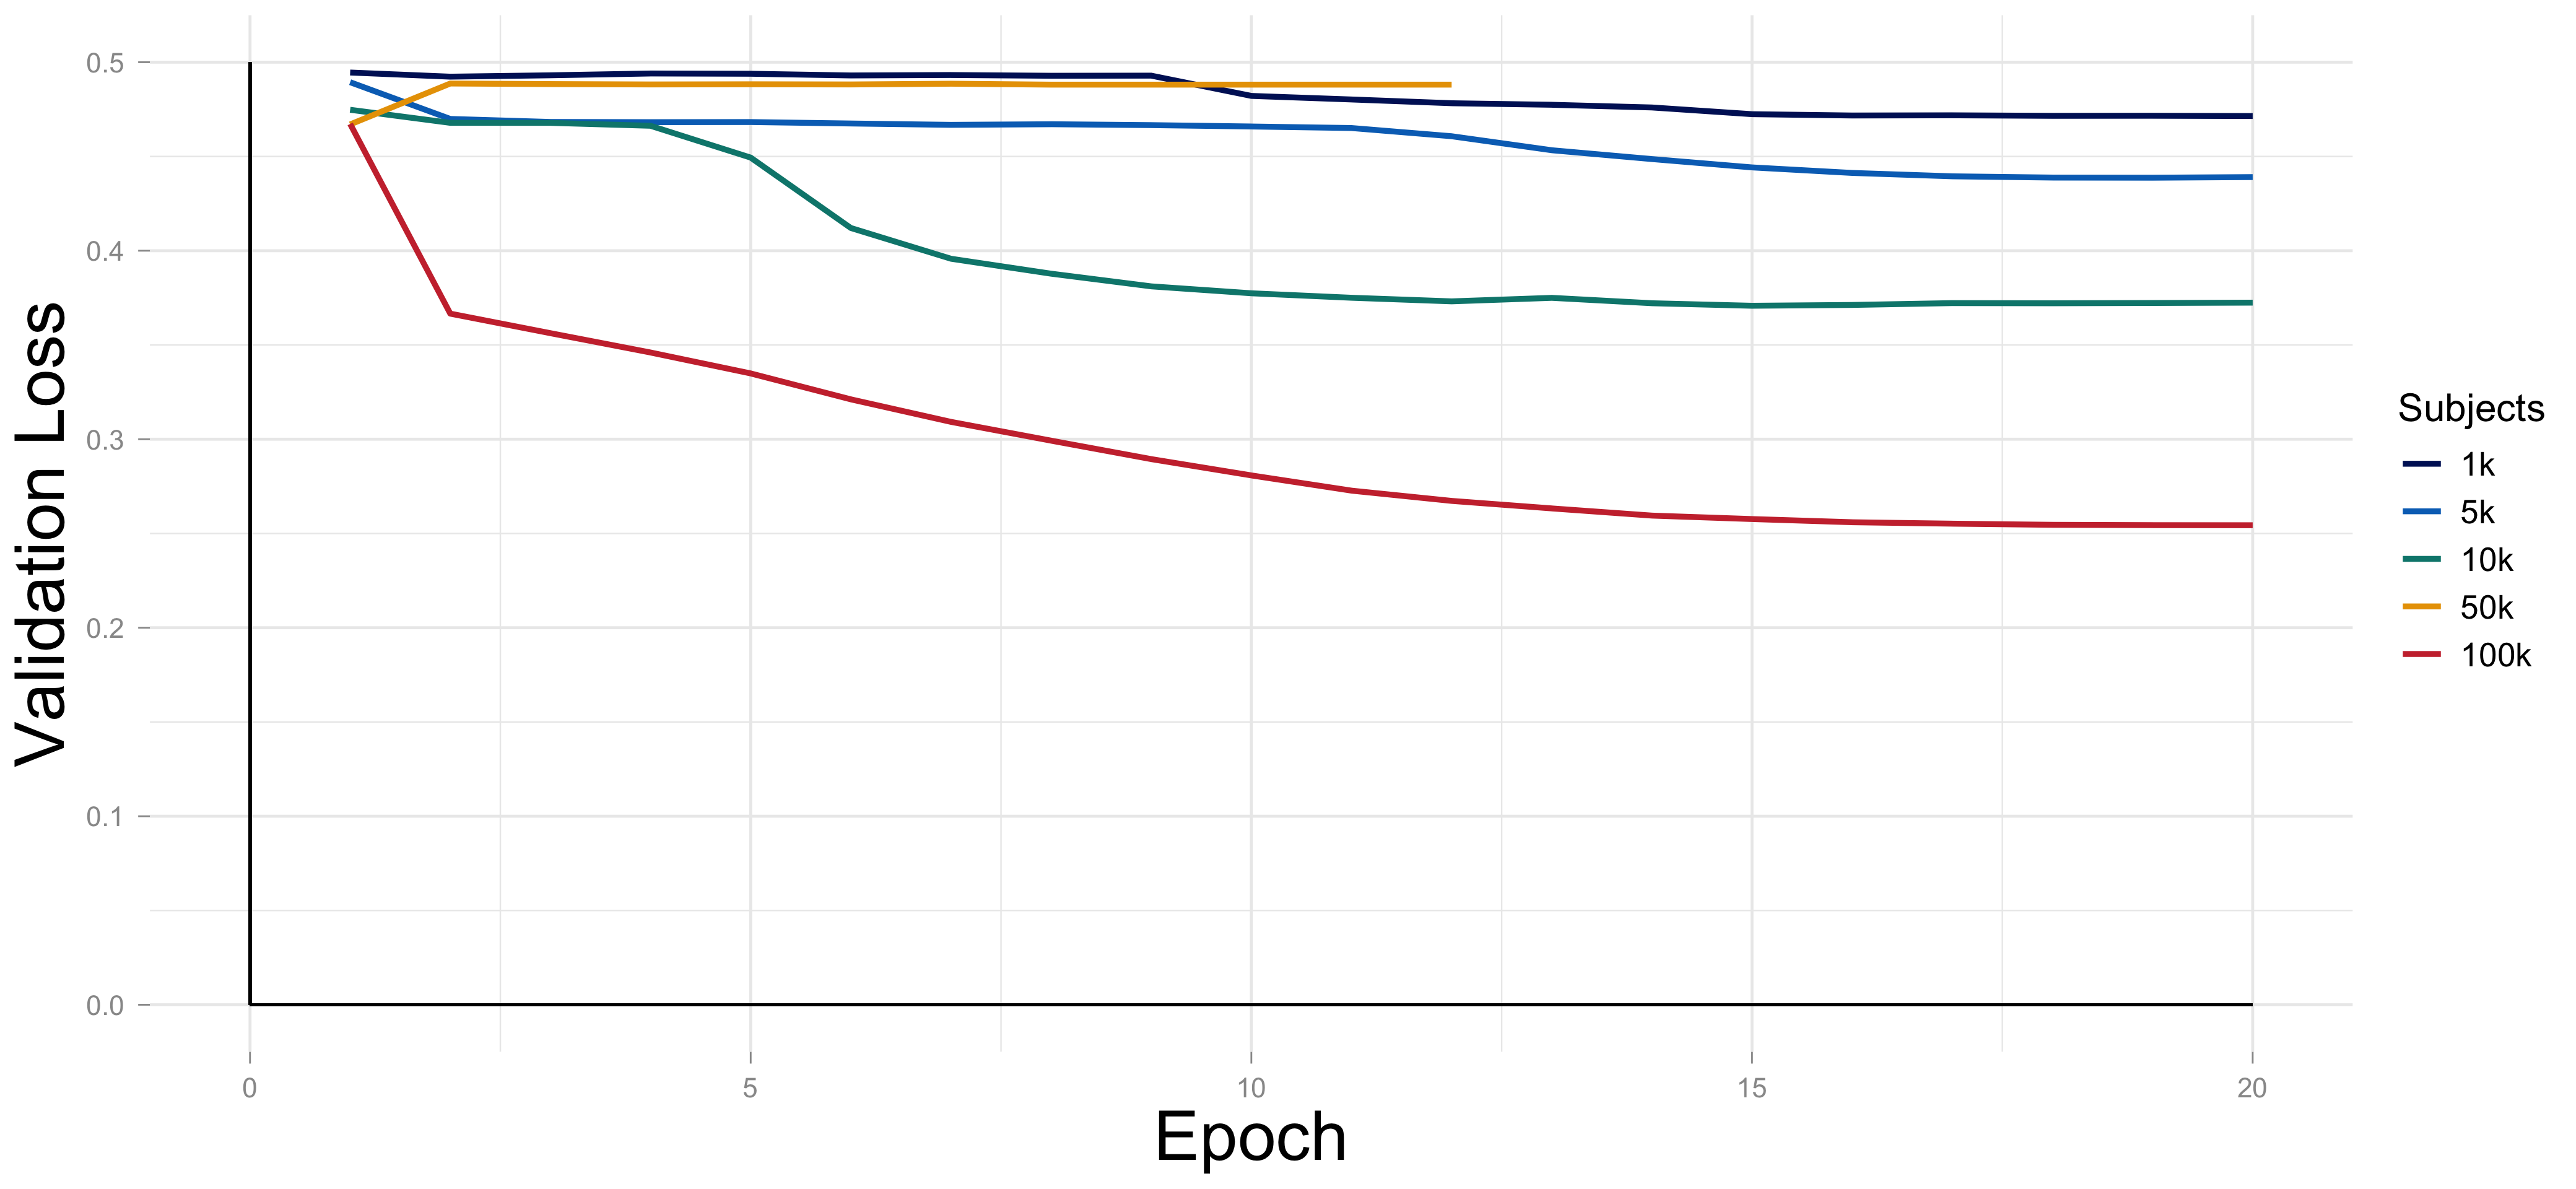
\includegraphics[width=0.95\linewidth]{fig/img/Pretrain/ValLoss.png}
    \caption{Validation loss during pre-training of SNPbag across different training set sizes. Each curve shows the masked cross-entropy loss on the validation set as a function of epoch, for training sets of $1000$, $5000$, $10000$, $50000, \text{and } 100000$ individuals. All runs use $M = 14000$ SNPs from chromosome~22, a mask probability of $0.85$, and $20$ epochs.}
    \label{fig:pretrain_val_loss}
\end{figure}

 
After pre-training, the SNPbag encoder has learned contextualised representations of genotype sequences from the masked genotype modelling objective without any phenotype information. Fine-tuning adapts these representations for binary phenotype prediction by replacing the masked genotype prediction head with a phenotype prediction head, as described in \autoref{sec:php}.
 
\subsection{Model Construction}

The fine-tuning model is constructed by loading the pre-trained encoder parameters with the lowest validation loss from the $100000$-individual run as the starting point of the prediction model.. The encoder and embedding architecture is identical to the pre-training configuration described in \autoref{tab:pretrain_hyperparams}. The masked genotype prediction head is discarded and replaced by a phenotype head, as described in \autoref{sec:php}.

Since the phenotype is defined for an entire individual rather than per-SNP, the encoder outputs are aggregated by mean pooling into a single vector per individual, which is passed to the phenotype head to obtain a predicted logit, as described in \autoref{sec:php}.
 
\subsection{Training Procedure}
\label{sec:app_finetune}
 %Freeze the encoder
Fine-tuning uses the same $70$/$10$/$20$ data split as LDpred2-auto, ensuring both methods are evaluated on identical individuals.
 
Due to a limited computational budget, the pre-trained encoder parameters are frozen during fine-tuning. This means that only the phenotype head is trained, while the encoder and embedding weights remain fixed at the values learned during pre-training. Freezing the encoder substantially decreases both the memory footprint and the time required per training step. The trade-off is that the encoder cannot adapt its representations to the phenotype prediction task, so the model relies entirely on the genomic context already captured during masked genotype pre-training.

Training was done for a single epoch with batch size $144$, distributed across $8$ GPUs, and the resulting model is evaluated on the test set using accuracy and AUC.

\section{Comparison of SNPbag and LDpred2-auto}
\label{sec:app_comparison}
 
Both methods are evaluated on the same test set $\mathcal{I}_{\text{test}}$ of $20000$ individuals using two metrics: classification accuracy at a threshold tuned on the validation set, and the area under the receiver operating characteristic curve (AUC). The results are summarised in \autoref{tab:comparison} and the ROC curves are shown in \autoref{fig:roc_comparison}.
 
\begin{table}[H]
\centering
\caption{Test set performance of LDpred2-auto and SNPbag on the simulated binary phenotype. The phenotype is simulated with the logistic disease model \citep{Majumdar2018} with $|\mathcal{M}_c| = 500$ causal SNPs, $\sigma_\beta = 0.5$, and a target prevalence of $K = 0.10$. Both methods are trained on $70\,000$ individuals, validated on $10\,000$ individuals, and tested on $20\,000$ individuals.}
\label{tab:comparison}
\begin{tabular}{l c c}
\toprule
\textbf{Method} & \textbf{Accuracy} & \textbf{AUC} \\
\midrule
LDpred2-auto & \texttt{0.507} & \texttt{0.510} \\
SNPbag       & \texttt{0.529} & \texttt{0.540} \\
\bottomrule
\end{tabular}
\end{table}

\begin{figure}[h]
    \centering
    \begin{subfigure}[t]{0.48\linewidth}
        \centering
        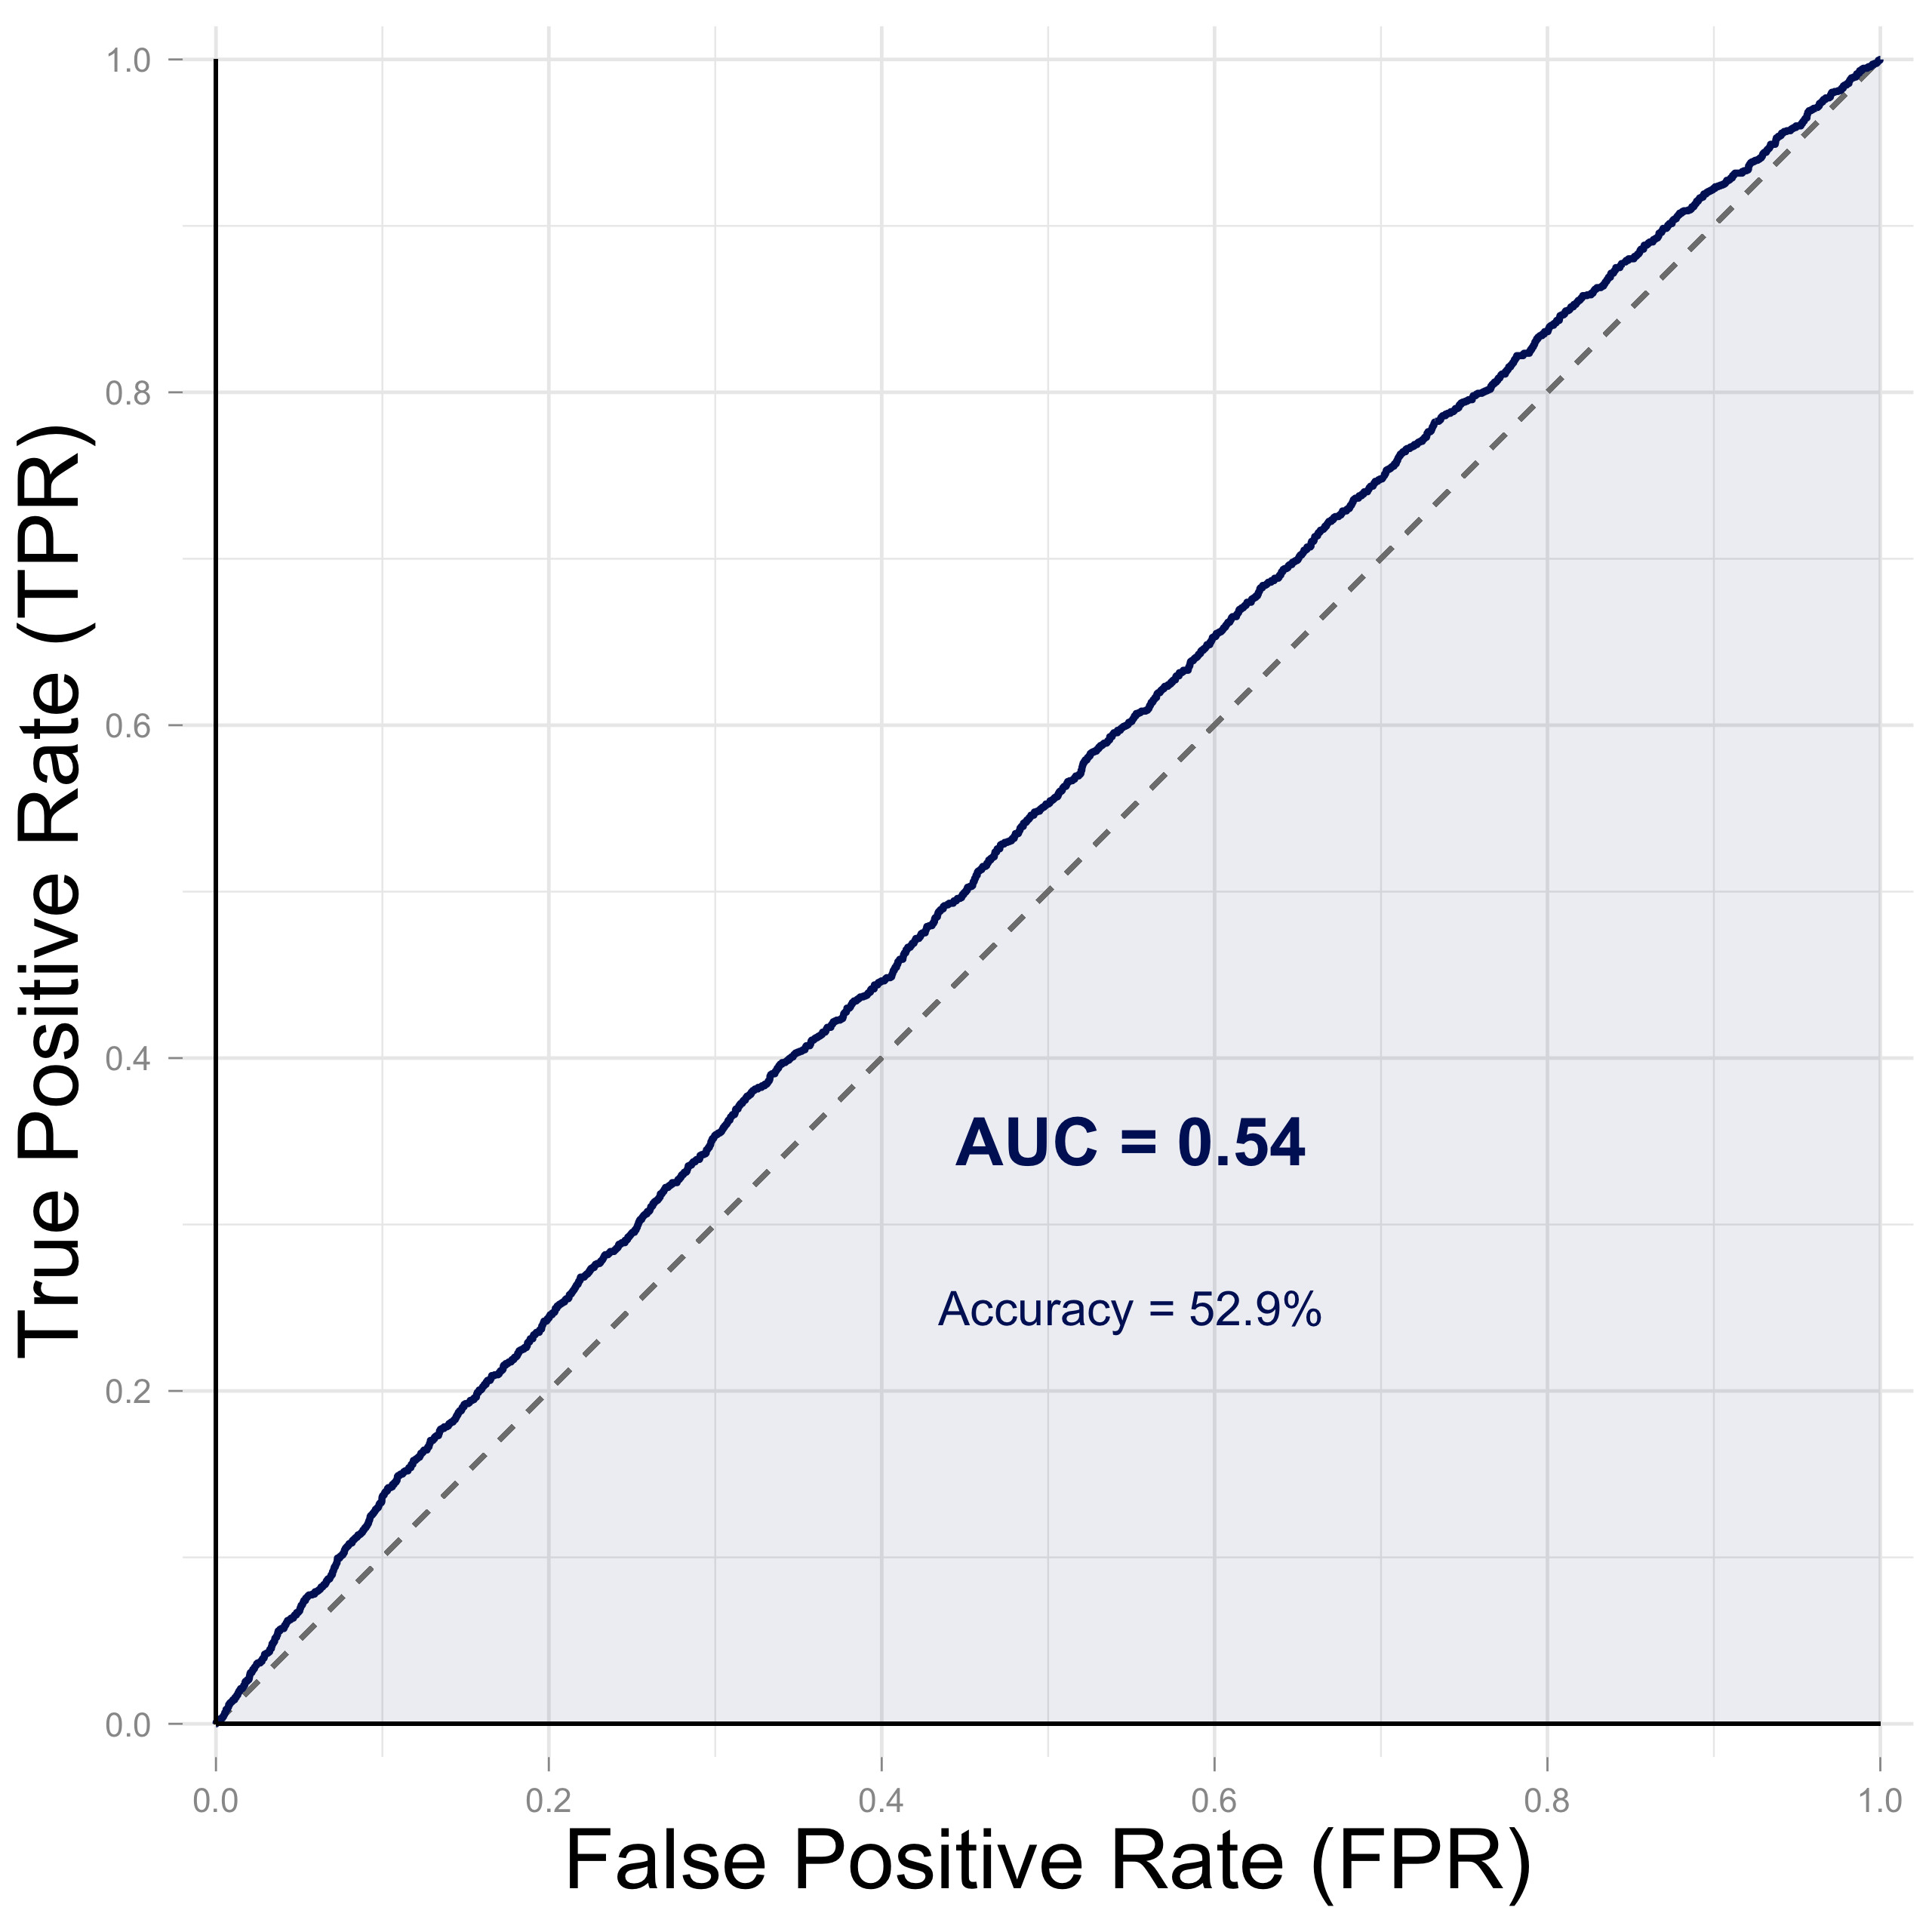
\includegraphics[width=\linewidth]{fig/img/SimStudy/ROC_SNPbag.png}
        \caption{SNPbag ($\mathrm{AUC} = 0.54$).}
        \label{fig:roc_snpbag}
    \end{subfigure}
    \hfill
    \begin{subfigure}[t]{0.48\linewidth}
        \centering
        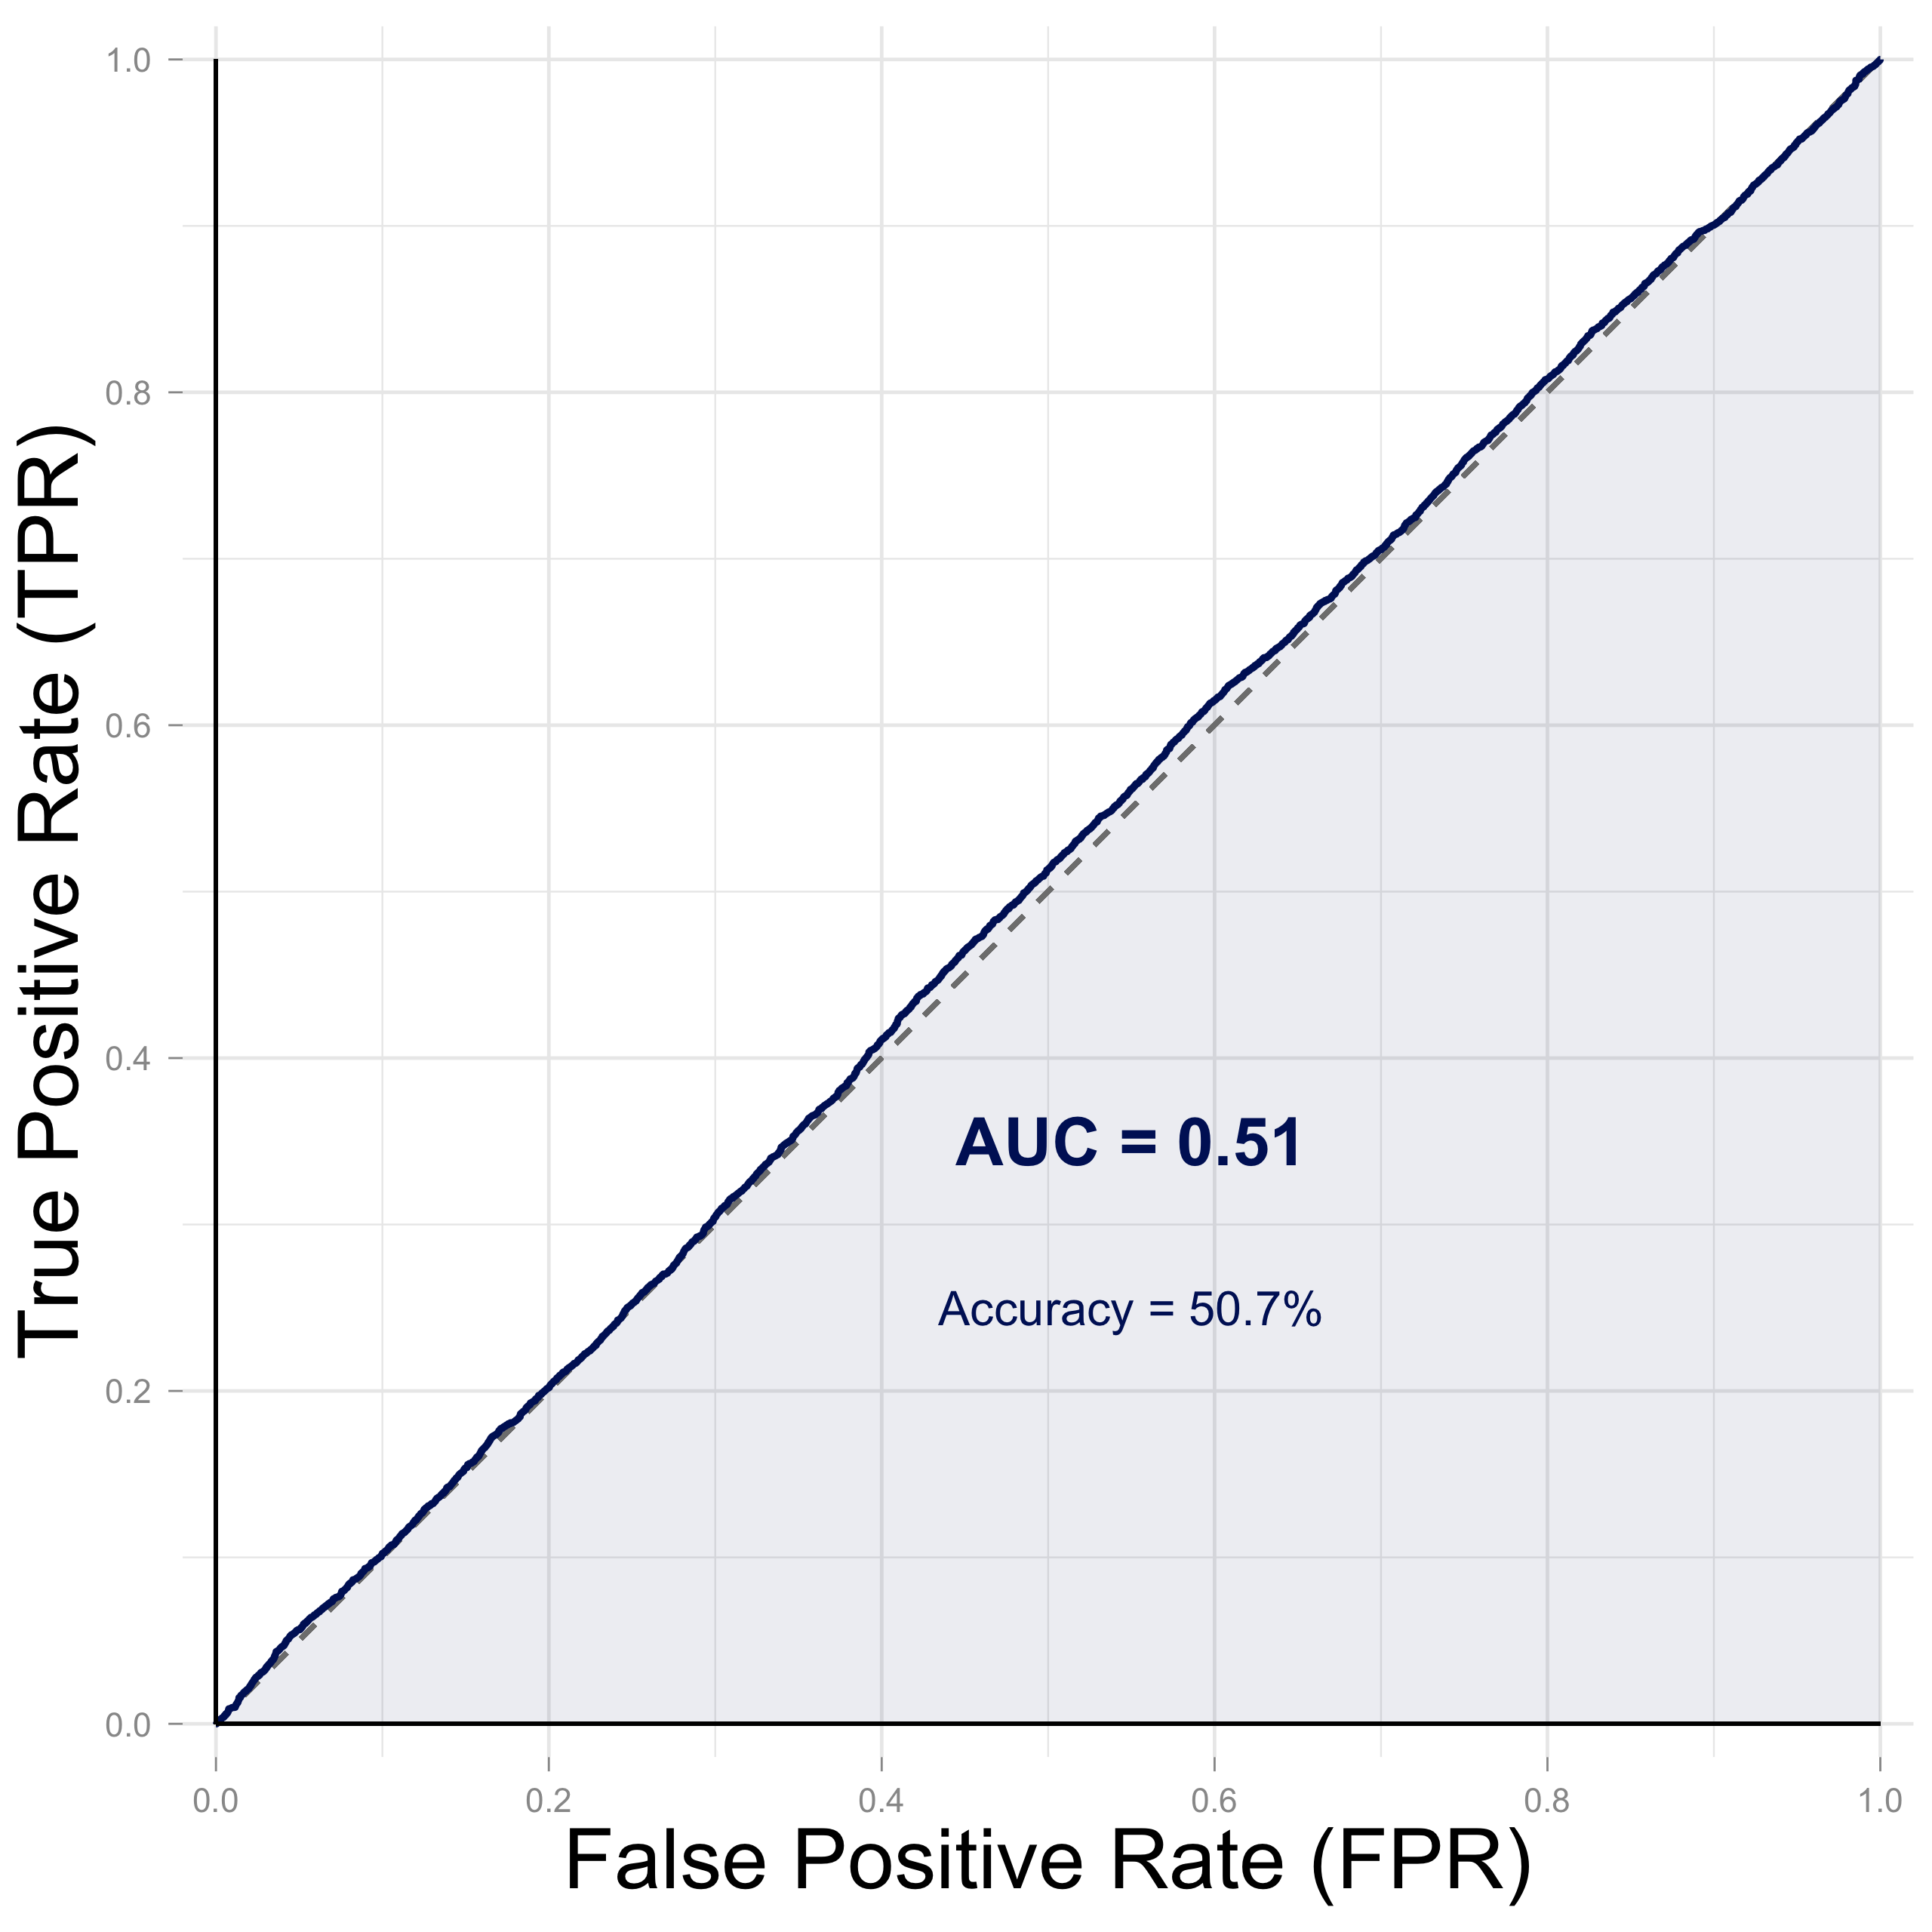
\includegraphics[width=\linewidth]{fig/img/SimStudy/ROC_GLM_LDpred2.png}
        \caption{LDpred2-auto ($\mathrm{AUC} = 0.51$).}
        \label{fig:roc_ldpred2}
    \end{subfigure}
    \caption{ROC curves on the test set for SNPbag and LDpred2-auto on the simulated binary phenotype described in \autoref{tab:comparison}. The shaded area corresponds to the AUC, and the dashed line represents a random classifier ($\mathrm{AUC} = 0.5$). Both curves lie close to the diagonal, indicating that neither method achieves meaningful discriminative power in this setting.}
    \label{fig:roc_comparison}
\end{figure}

The SNPbag achieved an accuracy of $52.9\%$, with an AUC of $0.54$, only slightly above the random baseline of $0.5$, which confirms that the model has minimal discriminative power. LDpred2-auto similarly shows a near-random AUC of $0.51$. Neither method achieved meaningful phenotype prediction in this setting. This is likely due to a combination of factors: SNPbag was limited to a single epoch with a frozen encoder, LDpred2-auto operated on only $14000$ SNPs from a single chromosome, and genotype-based prediction can at most explain the heritability $h^2$ of the trait, meaning that a substantial fraction of the phenotypic variation is driven by environmental factors that no genotype model can capture.
\chapter{Discussion}
\label{ch:discussion}

Neither SNPbag nor LDpred2-auto achieved meaningful discriminative
performance on the simulated phenotype, with AUCs of $0.54$ and $0.51$
respectively. The remainder of this chapter examines the limitations that
contributed to this outcome and identifies directions for future work.

The most significant limitation is the restricted genomic coverage.
The model was trained on only $14000$ SNPs from a single chromosome,
a constraint imposed entirely by GPU memory. Processing the full
chromosome~22 ($\sim\!116000$ SNPs) would exceed the memory of a
single NVIDIA B200 GPU even at the smallest batch size, and processing
all $22$ autosomes would require fundamentally different parallelisation
strategies. At the same time, the pre-training scaling experiment showed
that validation loss decreased monotonically as the training set grew
from $1000$ to $100000$ individuals, with the largest relative
improvement occurring between $10000$ and $100000$. This suggests
that the model has not yet saturated and would benefit from both longer
sequences and more training individuals.

All experiments were conducted on synthetic data generated by the HAPNEST
framework, not on real genotype data from a clinical cohort. While HAPNEST
preserves realistic linkage disequilibrium patterns and allele frequency
spectra, synthetic data may not fully capture the complexity of real human
genomes, including population substructure, rare variants, and genotyping
errors. The phenotype simulation used in this thesis assumes a simple
additive logistic model with a known set of causal variants, which may be
more favourable to both methods than the complex genetic architectures
underlying real diseases. Whether the pre-trained representations would
transfer to real data remains an open question.

Several architectural and methodological choices could be explored in
future work. SNPbag masks $85\%$ of genotype tokens during pre-training,
far higher than the $15\%$ used in the original BERT model
\citep{Devlin2019}. This aggressive masking forces the encoder to
reconstruct most of the sequence from very limited context, which may
strengthen the learned representations but could also make the
pre-training task unnecessarily difficult. The effect of the masking rate
on downstream phenotype prediction has not been investigated. Similarly,
the GELU activation function was inherited from the original BERT
architecture without exploration of alternatives such as SiLU or SwiGLU,
which have shown improvements in large language models. The prediction
head is a simple MLP applied to mean-pooled encoder output, and
alternative aggregation or prediction strategies could also be
considered. Each of these would require minimal code changes and could be
evaluated as straightforward ablation studies.

Finally, it is important to consider whether potential gains justify the
computational cost. Larger models and longer sequences may improve
prediction, but if the improvement is marginal or inconsistent across
traits, the added environmental and financial cost may not be worthwhile.
The results of this thesis suggest that the transformer architecture is
viable for learning genomic representations, the pre-training task
achieved $90\%$ masked accuracy, but that the current bottleneck is
scale, not architectural design.
\chapter{Conclusion}
\label{ch:conclusion}

This thesis developed SNPbag, a transformer-based model for phenotype
prediction from genotype data, and compared it against LDpred2-auto on
simulated binary phenotypes. The evaluation used $100000$ synthetic
individuals from the HAPNEST project with $14000$ SNPs from
chromosome~22 and phenotypes simulated under the logistic disease model
of \citet{Majumdar2018}.

The pre-training phase demonstrated that transformer-based self-supervised
learning can capture meaningful genomic structure. Masked genotype
prediction accuracy improved consistently from $84.18\%$ to $90.19\%$ as
the training set grew from $1000$ to $100000$ individuals, with
training and validation losses remaining close throughout, indicating no
overfitting. The continued improvement at $100000$ individuals suggests
the model has not yet saturated.

Despite effective pre-training, neither method achieved strong phenotype
prediction. SNPbag obtained an AUC of $0.54$ and LDpred2-auto an AUC of
$0.51$, both only marginally above the random baseline of $0.5$. Several
factors explain this. SNPbag was fine-tuned for a single epoch with a
frozen encoder, meaning the representations could not adapt to the
phenotype prediction task and the MLP had to learn the entire mapping from
fixed features in one pass. LDpred2-auto was designed for genome-wide
summary statistics but operated on only $14000$ SNPs from a single
chromosome, capturing a small fraction of the genetic variation it would
normally leverage. More fundamentally, genotype-based prediction is bounded
by the heritability $h^2$ of the trait, so a substantial fraction of the
phenotypic variation is driven by environmental factors that no genotype
model can capture. The combination of limited genomic coverage, restricted
fine-tuning, and the inherent heritability ceiling makes the near-random
performance unsurprising.

The key conclusion is that the bottleneck is scale, not architecture. The
pre-training results show that the transformer learns useful genomic
representations, and SNPbag achieved a marginally higher AUC than
LDpred2-auto despite operating under severe constraints. With greater
computational resources, future work could extend the model to longer
sequences, include more training individuals, and fine-tune the full
encoder, each of which addresses one of the limitations identified above.
% \include{incl/main/example2}
% ...

% Appendices are included inside an appendices block, which enumerates chapters
% with letters, starting from A, instead of numbers.
% \begin{appendices}
% \chapter{RNN}

Transformer models represent a fundamental advancement in the processing of sequential data, offering a highly parallelizable and effective alternative to traditional sequence models. These models are composed of multiple layers of attention and feed-forward mechanisms, enabling them to capture both local and global dependencies within sequences. The overall structure of a transformer model is illustrated in Figure (ref). While transformers have found broad application in domains such as natural language processing, speech recognition, and computer vision, this work specifically focuses on their adaptation for biological sequence analysis.

To provide a structured introduction, this chapter begins with a review of recurrent neural networks (RNNs), which formed the basis for sequence-to-sequence learning via encoder–decoder frameworks. Their limitations, particularly in handling long-range dependencies, motivate the transition to attention-based architectures. Subsequently, the chapter presents a stepwise development of the transformer model, followed by an explanation on how this general framework can be modified to accommodate the unique properties of biological sequences.

In addition, the chapter outlines training methodologies designed to optimize performance in this domain, considering aspects such as regularization, data augmentation, and optimization strategies. Finally, the chapter concludes with a detailed examination of evaluation metrics relevant to transformer-based models, highlighting criteria necessary for assessing predictive accuracy, generalization, and biological interpretability.


\section{Recurrent Neural Network and Backpropagation}
Consider a dataset consisting of $N \in \mathbb{N}$ sequences. Each sequence $i \in \{1, 2, \dots, N\}$ contains $n \in \mathbb{N}$ observations, $x_i = \{x_{i,1}, x_{i,2}, \dots, x_{i,n}\}$, and $q \in \N$ response variables, $y_i = \{y_{i,1}, y_{i,2}, \dots, y_{i,q}\}$. Collectively, all observation and response sequences yield the matrices $X = \{x_1, x_2, \dots, x_N \} \in \R^{N \times n}$ and $Y= \{y_1, y_2, \dots, y_N \} \in \R^{N \times q}$, respectively. A recurrent neural network (RNN) processes such sequences using hidden states to produce estimates based on the current and previous inputs, see Figure \ref{fig:example RNN}. The hidden state at each observation is defined recursively as
\begin{align*}
    h_{n} = f_\theta(h_{n-1}, x_n),
\end{align*}
where $h_n \in \R^p$ denotes the hidden state at observation $n$. The function $f_\theta : \R^{p} \times \R^N \to \R^{p}$ is an observation-invariant activation function parameterized by $\theta = \{ W, U, b_h\}$, where $W \in \R^{p\times p}$ is an invariant weight matrix between the hidden states, $U \in \R^{p \times N}$ is an invariant weight matrix between the inputs and the state, and $b_h \in \R^p$ is the bias between the states. Generally, the activation function used, is the hyperbolic tangent, at each entry of the vector. Thus, the hidden state at each observation can be described as
\begin{align*}
    h_n = \tanh(Wh_{n-1} + UX_{n-1} + b_h).
\end{align*}
Since $\tanh: \R \to (-1, 1)$, the resulting hidden state for the $n$'th observation $h_n \in (-1, 1)^p$. From each of the hidden states, an estimate can be obtained
\begin{align*}
    \hat{y}_n = g_\Theta(h_n),
\end{align*}
where $g_\Theta :\R^p \to \R^q$ is an invariant activation function parameterized by $\Theta = \{V, b_y\}$. Here $V \in \R^{q \times p}$ is a weight matrix between the hidden state and the output, and $b_y \in \R^q$ is a bias term. To represent the output as a probability distribution, the activation function, $g_\Theta (\cdot)$, is typically chosen to be the softmax function, yielding
\begin{align*}
    \hat{y}_{n,j} = \text{softmax}\left(Vh_n + b_y\right)= \frac{\exp((Vh_{n} + b_y)_j)}{\sum^q_{k=1}\exp((Vh_{n} + b_y)_k)},
\end{align*}
where $\hat{y}_{n,j}$ denotes the probability assigned to the j-th entry of the n-th input in the sequence. 
\begin{figure}
    \centering
    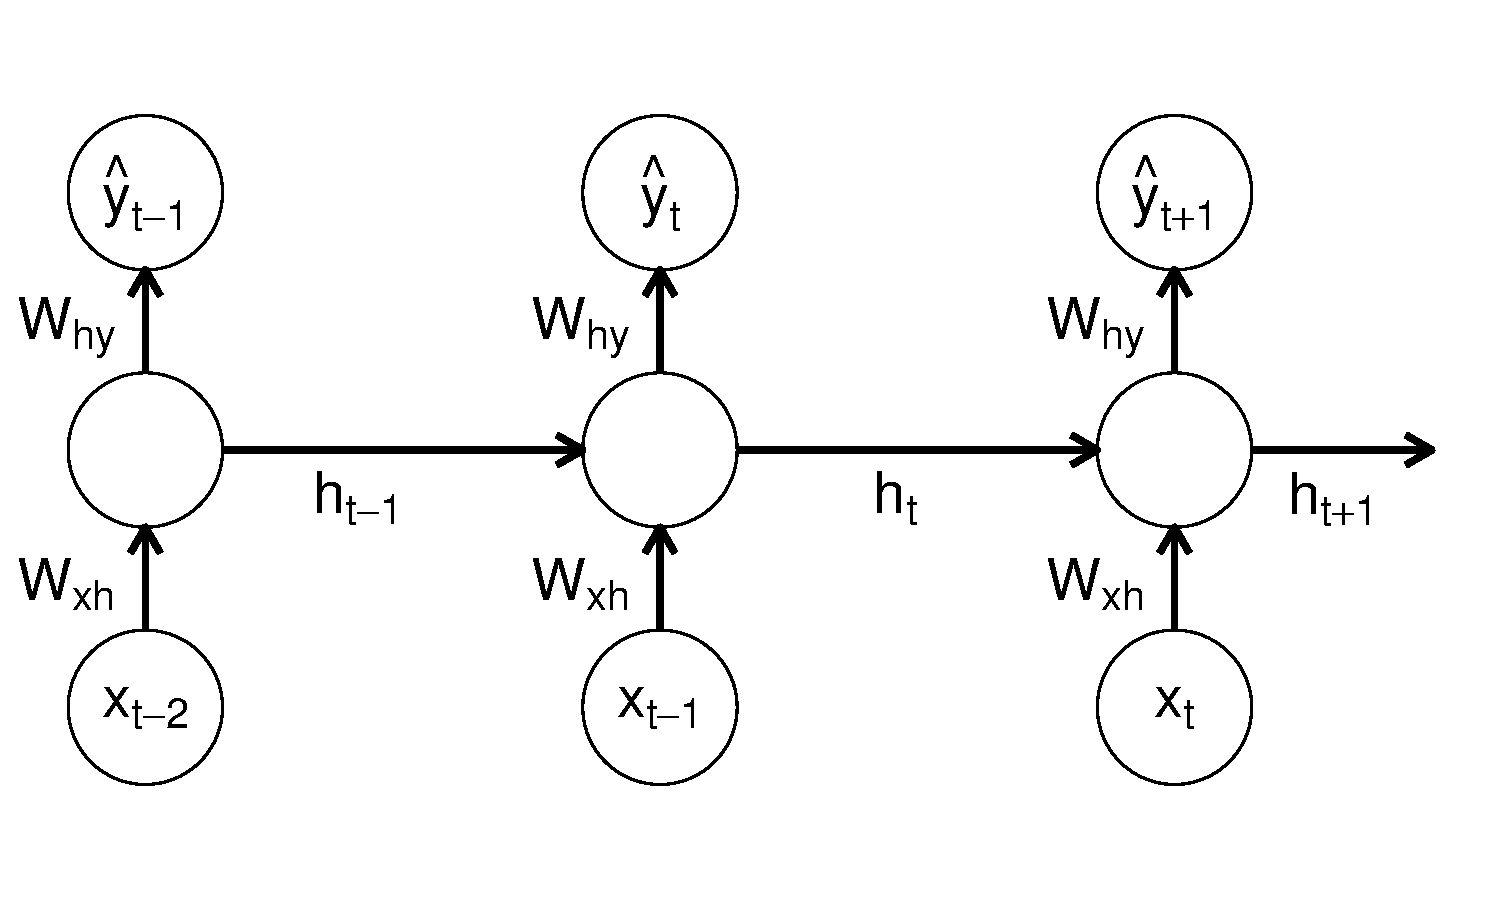
\includegraphics[width=0.8\linewidth]{fig/img/RNN/RNN_Example.pdf}
    \caption{Example of an RNN}
    \label{fig:example RNN}
\end{figure}


%   % \include{incl/app/appendix2}
%   % ..
% \end{appendices}

% The backmatter is for extra stuff. Headings are not numbered.
\backmatter

% Automatic list of references, based on which references in the literature
% database files were referenced throughout the document.
\bibliographystyle{apalike}
\label{bib}
\bibliography{
  incl/bib/books,
  incl/bib/articles,
  incl/bib/software,
  incl/bib/references
}

\end{document}
